\documentclass[modern]{aastex62}

\pdfoutput=1

%\usepackage{lmodern}
%\usepackage{microtype}
\usepackage{url}
\usepackage{amsmath}
\usepackage{amssymb}
\usepackage{natbib}
\usepackage{multirow}
\usepackage{graphicx}
\bibliographystyle{aasjournal}

\usepackage{mathtools}
\usepackage{calc}
\usepackage{etoolbox}
\usepackage{xspace}
\usepackage[T1]{fontenc} % https://tex.stackexchange.com/a/166791
\usepackage{textcomp}
\usepackage{ifxetex}
\ifxetex
\usepackage{fontspec}
\defaultfontfeatures{Extension = .otf}
\fi
\usepackage{fontawesome}

% Matrix fix:
% http://tex.stackexchange.com/questions/317824/letter-c-appearing-inside-pmatrix-environment-with-aastex
\makeatletter
\def\env@matrix{\hskip -\arraycolsep\let\@ifnextchar\new@ifnextchar\array{*{\c@MaxMatrixCols}c}}
\makeatother

% Column spacing in matrix
% http://tex.stackexchange.com/questions/275725/adjusting-separation-between-matrix-entries
\setlength\arraycolsep{25pt}

% ------------------ %
% end of AASTeX mods %
% ------------------ %

% Projects:
\newcommand{\project}[1]{\textsf{#1}}
\newcommand{\exoplanet}{\project{exoplanet}}
\newcommand{\starry}{\project{starry}}
\newcommand{\radvel}{\project{RadVel}}
\newcommand{\batman}{\project{batman}}
\newcommand{\python}{\project{Python}}
\newcommand{\cython}{\project{Cython}}
\newcommand{\cpp}{\project{C++}}
\newcommand{\theano}{\project{Theano}}
\newcommand{\pymc}{\project{PyMC3}}
\newcommand{\pytorch}{\project{PyTorch}}
\newcommand{\tensorflow}{\project{TensorFlow}}
\newcommand{\stan}{\project{Stan}}
\newcommand{\celerite}{\project{celerite}}
\newcommand{\tess}{\project{TESS}}


% references to text content
\newcommand{\documentname}{\textsl{Note}}
\newcommand{\figureref}[1]{\ref{fig:#1}}
\newcommand{\Figure}[1]{Figure~\figureref{#1}}
\newcommand{\figurelabel}[1]{\label{fig:#1}}
\renewcommand{\eqref}[1]{\ref{eq:#1}}
\newcommand{\Eq}[1]{Equation~(\eqref{#1})}
\newcommand{\eq}[1]{\Eq{#1}}
\newcommand{\eqalt}[1]{Equation~\eqref{#1}}
\newcommand{\eqlabel}[1]{\label{eq:#1}}

% TODOs
\newcommand{\todo}[3]{{\color{#2}\emph{#1}: #3}}
\newcommand{\dfmtodo}[1]{\todo{DFM}{red}{#1}}
\newcommand{\alltodo}[1]{\todo{TEAM}{red}{#1}}
\newcommand{\citeme}{{\color{red}(citation needed)}}

% math
\newcommand{\T}{\ensuremath{\mathrm{T}}}
\newcommand{\dd}{\ensuremath{ \mathrm{d}}}
\newcommand{\unit}[1]{{\ensuremath{ \mathrm{#1}}}}
\newcommand{\bvec}[1]{{\ensuremath{\boldsymbol{#1}}}}

% typography obsessions
\setlength{\parindent}{3.0ex}

% from: https://github.com/rodluger/corTeX
% Add code, proof, and animation hyperlinks
\definecolor{linkcolor}{rgb}{0.1216,0.4667,0.7059}
\newcommand{\codeicon}{{\color{linkcolor}\faFileCodeO}}
\newcommand{\prooficon}{{\color{linkcolor}\faPencilSquareO}}
\newcommand{\codelink}[1]{\href{https://github.com/dfm/exoplanet/blob/3f5ce20d413f052d603c156162e3d0b95204367c/paper/figures/#1.ipynb}{\codeicon}\,\,}
\newcommand{\animlink}[1]{\href{https://github.com/dfm/exoplanet/blob/3f5ce20d413f052d603c156162e3d0b95204367c/paper/figures/#1.gif}{\animicon}\,\,}
\newcommand{\prooflink}[1]{\href{https://github.com/dfm/exoplanet/blob/3f5ce20d413f052d603c156162e3d0b95204367c/paper/proofs/#1.ipynb}{\raisebox{-0.1em}{\prooficon}}}


% Define a proof environment for open source equation proofs
\newtagform{eqtag}[]{(}{)}
\newcommand{\currentlabel}{None}
\newenvironment{proof}[1]{%
\ifstrempty{#1}{%
\renewtagform{eqtag}[]{\raisebox{-0.1em}{{\color{red}\faPencilSquareO}}\,(}{)}%
}{%
\renewtagform{eqtag}[]{\prooflink{#1}\,(}{)}%
}%
\usetagform{eqtag}%
\renewcommand{\currentlabel}{#1}
\align%
}{%
\endalign%
\renewtagform{eqtag}[]{(}{)}%
\usetagform{eqtag}%
\message{<<<\currentlabel: \theequation>>>}%
}

% Define the `oscaption` command for open source figure captions
\newcommand{\oscaption}[2]{\caption{#2 \codelink{#1}}}

\newcommand{\Gaussian}[3]{\ensuremath{\frac{1}{|2\pi #2|^\frac{1}{2}}
            \exp\left[ -\frac{1}{2}#1^\top #2^{-1} #1 \right]}}

\newcommand{\Normal}{\ensuremath{\mathcal{N}}}
\newcommand{\mA}{\ensuremath{\bvec{A}}}
\newcommand{\mC}{\ensuremath{\bvec{C}}}
\newcommand{\mS}{\ensuremath{\bvec{\Sigma}}}
\newcommand{\mL}{\ensuremath{\bvec{\Lambda}}}
\newcommand{\vw}{\ensuremath{\bvec{w}}}
\newcommand{\vy}{\ensuremath{\bvec{y}}}
\newcommand{\vt}{\ensuremath{\bvec{\theta}}}
\newcommand{\vm}{\ensuremath{\bvec{\mu}(\bvec{\theta})}}
\newcommand{\vre}{\ensuremath{\bvec{r}}}
\newcommand{\vh}{\ensuremath{\bvec{h}}}
\newcommand{\vk}{\ensuremath{\bvec{k}}}


\begin{document}\raggedbottom\sloppy\sloppypar\frenchspacing

\title{%
\project{exoplanet}:
A toolkit for scalable inference for exoplanetary systems using transits,
radial velocities, \& astrometry
%An efficient and robust toolkit for gradient-based
%probabilistic characterization of exoplanets using transits and radial
%velocities
}

\author[0000-0002-9328-5652]{Daniel Foreman-Mackey}
\affil{Center for Computational Astrophysics, Flatiron Institute, New York, NY}

\begin{abstract}

As larger and more precise datasets continue to be collected for the discovery
and characterization of exoplanets, we must also develop computationally
efficient and rigorous methods for making inferences based on these data.
The efficiency and robustness of numerical methods for probabilistic inference
can be improved by using derivatives of the model with respect to the
parameters.
In this paper, I derive methods for exploiting these gradient-based methods
when fitting exoplanet data based on radial velocity, astrometry, and
transits.
Alongside the paper, I release an open source, well-tested, and
computationally efficient implementation of these methods.
These methods can substantially reduce the computational cost of fitting large
datasets and systems with more than one exoplanet.

\end{abstract}

\keywords{%
methods: data analysis ---
methods: statistical
}

\section{Outline}

\begin{enumerate}

{\item Introduction
\begin{itemize}
{\item the datasets available and forthcoming}
{\item existing tools for exoplanet fitting}
{\item motivation for gradients}
\end{itemize}}

\item Automatic differentiation and inference frameworks

\item Hamiltonian Monte Carlo and variants

\item Custom gradients required for exoplanet datasets
\begin{itemize}
\item Radial velocities and Kepler's equation
\item Astrometry
\item Transits
\end{itemize}

\item Implementation details and benchmarks

\item Examples

\item Discussion

\end{enumerate}

\section{Introduction}

Datasets are getting larger and more precise and this leads to an interest in
more ambitious questions about these systems.
The existing inference methods are no longer up to the task when the datasets
are large and when the number of parameters is large.
Many probabilistic inferences in astronomy have been limited by the existing
tools that can't scale e.g.\ emcee.
However, in other fields such as ML, methods have been developed that can
scale to datasets too large to fit into memory and millions of parameters.
The key ingredient in all of these methods is that it must be possible to
efficiently evaluate the derivative of the model with respect to the physical
parameters.
This can often be intractable for applications astrophysics because the models
generally include a physically motivated component that can't be trivially
differentiated.
However, we can take advantage of the substantial development that has been
invested in automating this process.

This paper presents an example of how these tools and methods can be
exploited in the specific astronomical application of fitting exoplanet
datasets.
We go through the derivation and implementation of the custom functions and
their gradients that are required for gradient-based characterization of
exoplanets.

These methods and their implementation are not an all-in-one package designed
to do the fitting.
Instead, it provided the framework needed to use these tools within pipelines.

\begin{figure}[htbp]
\begin{centering}
\includegraphics[width=0.8\linewidth]{figures/simple_rv.pdf}
\oscaption{simple_rv}{\label{fig:simple_rv}
This is a figure.}
\end{centering}
\end{figure}

\section{Automatic differentiation}

The main limitation of gradient-based inference methods is that, in order to
use them, you must \emph{compute the gradients}!
The fundamental quantity of interest is the first derivative (gradient) of the
log-likelihood function (or some other goodness-of-fit function) with respect
to the parameters of the model.
In all but the simplest cases, symbolically deriving this gradient function is
tedious and error-prone.
Instead, it is generally preferable to use a method (called automatic
differentiation) that can automatically compute the exact gradients of the
model \emph{to machine precision} at compile time.
We would like to emphasize the fact that we are not talking \emph{numerical}
derivatives like finite difference methods, and there is no approximation
being made.

The basic idea behind automatic differentiation is that code is always written
as the composition of basic functions and, if we know how to differentiate the
subcomponents, then we can apply the chain rule to differentiate the larger
function.
This realization was one of the key discoveries that launched the field of
machine learning called ``deep learning'', where automatic differentiation was
given the name ``backpropagation'' (CITE).
Since then, there has been a substantial research base that has made these
methods general and computationally efficient, and from this, many open source
libraries have been released that ease the use of these methods (e.g.\
TensorFlow, PyTorch, Stan, ceres, Eigen, etc.\ CITATIONS).
Despite the existence of these projects, automatic differentiation has not
been widely adopted in the astronomical literature because there is some
learning curve associated with porting existing code bases to a new language
or framework.
Furthermore, many projects in astronomy involve fitting realistic, physically
motivated models that involve numerical solutions to differential equations
or special functions that are not natively supported by the popular automatic
differentiation frameworks.

In this paper, we demonstrate how to incorporate exoplanet-specific functions
into these frameworks and derive the functions needed to characterize
exoplanets using gradient-based methods applied to radial velocity,
astrometry, and transit datasets.
Similar derivations would certainly be tractable for microlensing, direct
imaging, and other exoplanet characterization methods, but these are left to a
future paper.

At present, there are many model-building libraries available in every
programming language, and it is not clear which should be preferred.
For this paper, we focus on implementations within TensorFlow
\citep{Abadi:2016} because it is accessible using Python, the most widely used
programming language in astronomy (CITE?) and because the code is
well-supported and stable.
This being said, the basic ideas behind each library are similar and the core
implementation in C++ can be minimally modified to support other frameworks.

\section{The custom operations provided by exoplanet}

\subsection{A solver for Kepler's equation}

A key assumption that is often made when fitting exoplanets is that the
planets are orbiting the central star on independent bound Keplerian orbits
(CITE).
To compute the coordinates of a planet on its orbit, we must solve Kepler's
equation
\begin{eqnarray}
M &=& E - e\,\sin E
\end{eqnarray}
for the eccentric anomaly $E$ at fixed eccentricity $e$ and mean anomaly $M$.
This equation must be solved numerically and there is a rich literature
discussing methods for this implementation.
We have found the method from CITE to provide the right balance of numerical
stability (with a relative accuracy of about $10^{-20}$ for all values of $M$
and $e$) and computational efficiency.

As well as solving Kepler's equation, we must also efficiently evaluate the
gradients (or, more precisely, \emph{back-propagate} the gradients) of $E$
with respect to $e$ and $M$.
After solving for $E$, this can be computed efficiently and robustly using
implicit differentiation.
For numerical methods like this, it is often possible to compute the gradients
without applying automatic differentiation to the implementation directly and
that is generally preferred for the purposes of numerical stability.
In this case, the relevant gradients are
\begin{eqnarray}
\frac{\dd E}{\dd e} &=& \frac{\sin E}{1 - e\,\cos E} \\
\frac{\dd E}{\dd M} &=& \frac{1}{1 - e\,\cos E} \quad.
\end{eqnarray}

\paragraph{Implementation details}

We find that directly evaluating the true anomaly $f$
%\begin{eqnarray}
%f &=& 2\,\tan^{-1}\,left(\frac{\sqrt{1+e}}{\sqrt{1-e}}\,\tan \frac{E}{2}\right)
%\end{eqnarray}
when solving Kepler's equation is more efficient than evaluating it separately
within Theano.
This means that we must also provide a method for evaluating the derivative of
$f$ with respect to $e$ and $M$.

\begin{figure}[htbp]
\begin{centering}
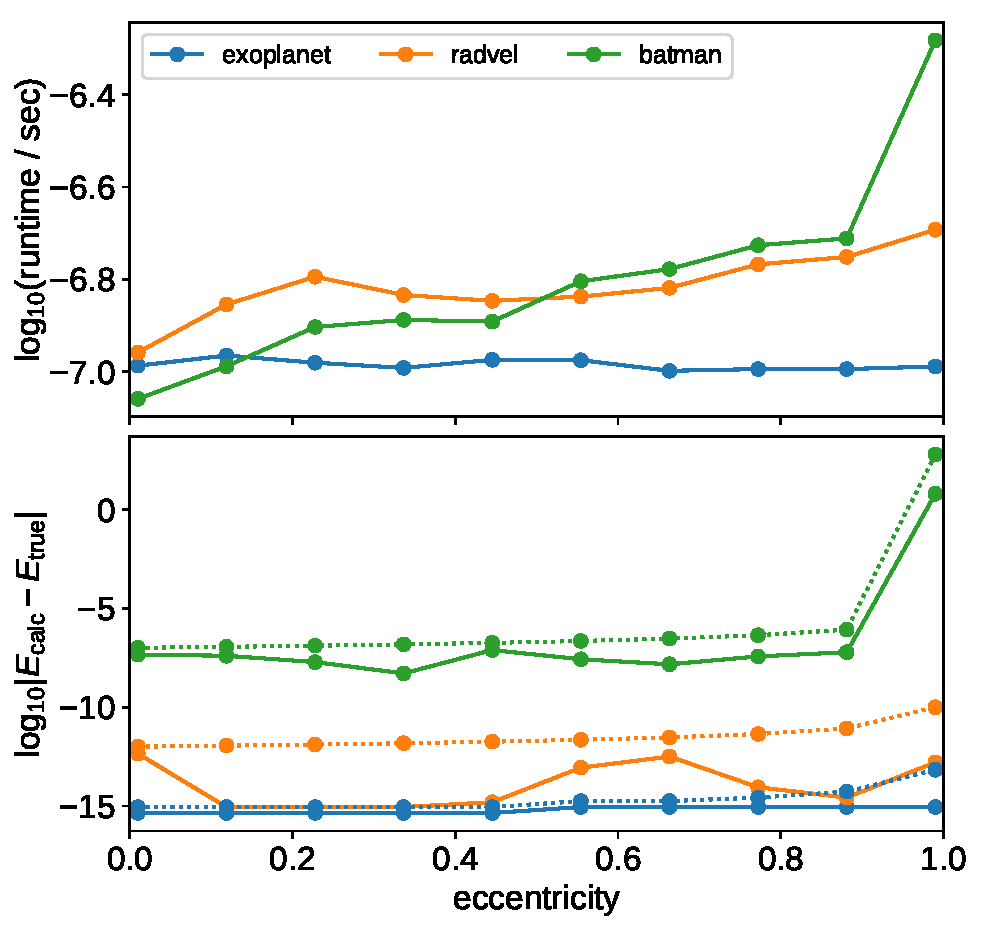
\includegraphics[width=0.8\linewidth]{figures/kepler_solver.pdf}
\oscaption{kepler_solver}{\label{fig:kepler_solver}
The performance of the Kepler solver used by \exoplanet\ compared to
the solvers from the \radvel\ \citep{Fulton:2017, Fulton:2018} and \batman\
\citep{Kreidberg:2015} libraries.
\emph{top}: The average wall time required to solve Kepler's equation once for
the eccentric anomaly $E$ conditioned on eccentricity $e$ and mean anomaly $M$.
Smaller numbers correspond to faster solutions.
\emph{bottom}: The 90-th percentile of the absolute error of the computed
eccentric anomaly for 5000 true values of $E$ in the range $0 \le E < 2\,\pi$.
Smaller numbers correspond to more accurate solutions.}
\end{centering}
\end{figure}


\subsection{Limb-darkened light curves}

\subsection{Scalable Gaussian Processes for time series}

\appendix

\section{Contact points}

In the plane of the orbit, $S_0$, the coordinates of the orbit satisfy the
equation
\begin{eqnarray}\eqlabel{constraint0}
{({x_0} - a\,e)}^2 + \frac{{y_0}^2}{1-e^2} &=& a^2 \quad.
\end{eqnarray}
To rotate into the observing plane, we perform the following transformation
\begin{eqnarray}\eqlabel{rotation}
\bvec{x}_2 &=& R_i\,R_\omega\,\bvec{x}_0 \\
\left(\begin{array}{c}x_2\\y_2\\z_2\end{array}\right) &=&
\left(\begin{array}{ccc}
1 & 0 & 0\\
0 & \cos i & \sin i \\
0 & -\sin i & \cos i \\
\end{array}\right) \,
\left(\begin{array}{ccc}
\cos\omega & \sin\omega & 0\\
-\sin\omega & \cos\omega & 0 \\
0 & 0 & 1 \\
\end{array}\right) \,
\left(\begin{array}{c}x_0\\y_0\\0\end{array}\right) \quad.
\end{eqnarray}
In this space, the planet will transit whenever
\begin{eqnarray}
z_2 < 0 &\mathrm{and}& {x_2}^2 + {y_2}^2 < L^2
\end{eqnarray}
where $L = R_\star + R_P$.
The contact point therefore occurs when
\begin{eqnarray} \eqlabel{quad1}
\hat{x_2}^2 + \hat{y_2}^2 = L^2
\end{eqnarray}
where the hat indicates that

Using the inverse of \eq{rotation} to re-write \eq{constraint0} in terms of
$x_2$ and $y_2$, we find the following quadratic equation
\begin{eqnarray} \eqlabel{quad2}
A\,{x_2}^2 + B\,{x_2\,y_2} + C\,{y_2}^2 + D\,x_2 + E\,y_2 + F &=& 0
\end{eqnarray}
with
\begin{eqnarray}
A &=& \left(e^{2}\,\cos^{2}{\omega} - 1\right)\,\cos^{2}{i} \\
B &=& 2\,e^{2}\,\cos{i}\,\sin{\omega}\,\cos{\omega}\\
C &=& e^{2}\,\sin^{2}{\omega} - 1\\
D &=& 2\,a\,e\,\left(1-e^{2}\right)\,\cos^{2}{i}\,\cos{\omega}\\
E &=& 2\,a\,e\,\left(1-e^{2}\right)\,\sin{\omega} \cos{i}\\
F &=& a^{2}\,\left(e^{2} - 1\right)^{2}\,\cos^{2}{i}
\end{eqnarray}

The pair of quadratic equations defined by \eq{quad1} and \eq{quad2} can be
combined to give a quartic equation for $x_2$
\begin{eqnarray}
a_0 + a_1\,{x_2} + a_2\,{x_2}^2 + a_3\,{x_2}^3 + a_4\,{x_2}^4 = 0
\end{eqnarray}
where
\begin{eqnarray}
a_0 &=& \left(C L^{2} - E L + F\right) \left(C L^{2} + E L + F\right) \\
a_1 &=& - 2 \left(B E L^{2} - C D L^{2} - D F\right)\\
a_2 &=& 2 A C L^{2} + 2 A F - B^{2} L^{2} - 2 C^{2} L^{2} - 2 C F + D^{2} + E^{2}\\
a_3 &=& 2 \left(A D + B E - C D\right)\\
a_4 &=& A^{2} - 2 A C + B^{2} + C^{2}
\end{eqnarray}
which can be solved symbolically (CITE Kipping) or numerically.

\paragraph{Edge-on orbits}
For an edge-on orbit, $\cos{i} = 0$ and the contact points occur at
\begin{eqnarray}\eqlabel{edgeon1}
x_2 &=& \pm L \\
y_2 &=& 0 \quad,
\end{eqnarray}
but care must be taken when evaluating $z_2$.
To do this, we substitute \eq{edgeon1} into \eq{constraint0} to get the
following quadratic equation for $z_2$
\begin{eqnarray}
b_0 + b_1\,{z_2} + b_2\,{z_2}^2 &=& 0
\end{eqnarray}
where
\begin{eqnarray}
b_{0,\pm} &=& L^2\,(e^2\,\cos^2\omega - 1) \mp 2\,a\,e\,L\,\cos\omega\,(e^2-1) +
a^2\,{(e^2 -1)}^2 \\
b_{1,\pm} &=& -2\,a\,e\,\sin\omega\,(e^2-1) \pm 2\,e^2\,L\,\sin\omega\,\cos\omega\\
b_{2,\pm} &=& e^{2} \sin^{2}{\left (\omega \right )} - 1 \quad.
\end{eqnarray}
There are 4 solutions to this system of which we are only interested in the
ones where $z_2 < 0$ (the others are the contact points for the occultation).

\begin{figure}[htbp]
\begin{centering}
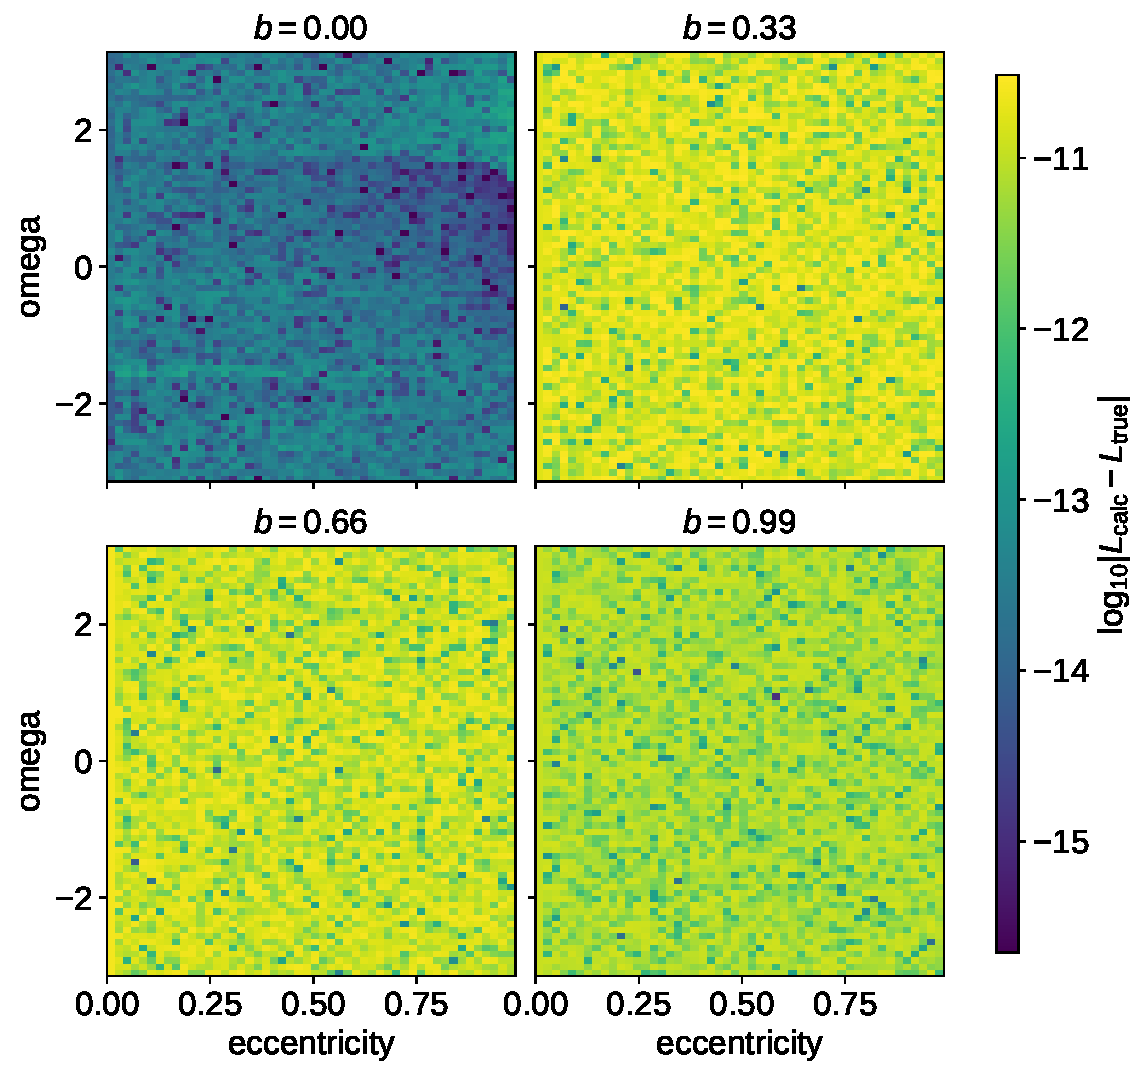
\includegraphics[width=0.8\linewidth]{figures/contact_points.pdf}
\oscaption{contact_points}{\label{fig:contact_points}
This is a figure.}
\end{centering}
\end{figure}

\newpage
\bibliography{exoplanet}


\end{document}
